
\section*{Anhang A} \label{appA}

	\noindent\textit{Materialien zur Bestimmung der US-Intensität:} (1) \textit{Skala zur Einschätzung der US-Intensität,} (2) \textit{Tabelle zur Kalibrierung der individuellen Reizintensität}
	
	\vspace*{2cm}
	\noindent\begin{minipage}[t]{14cm}
		 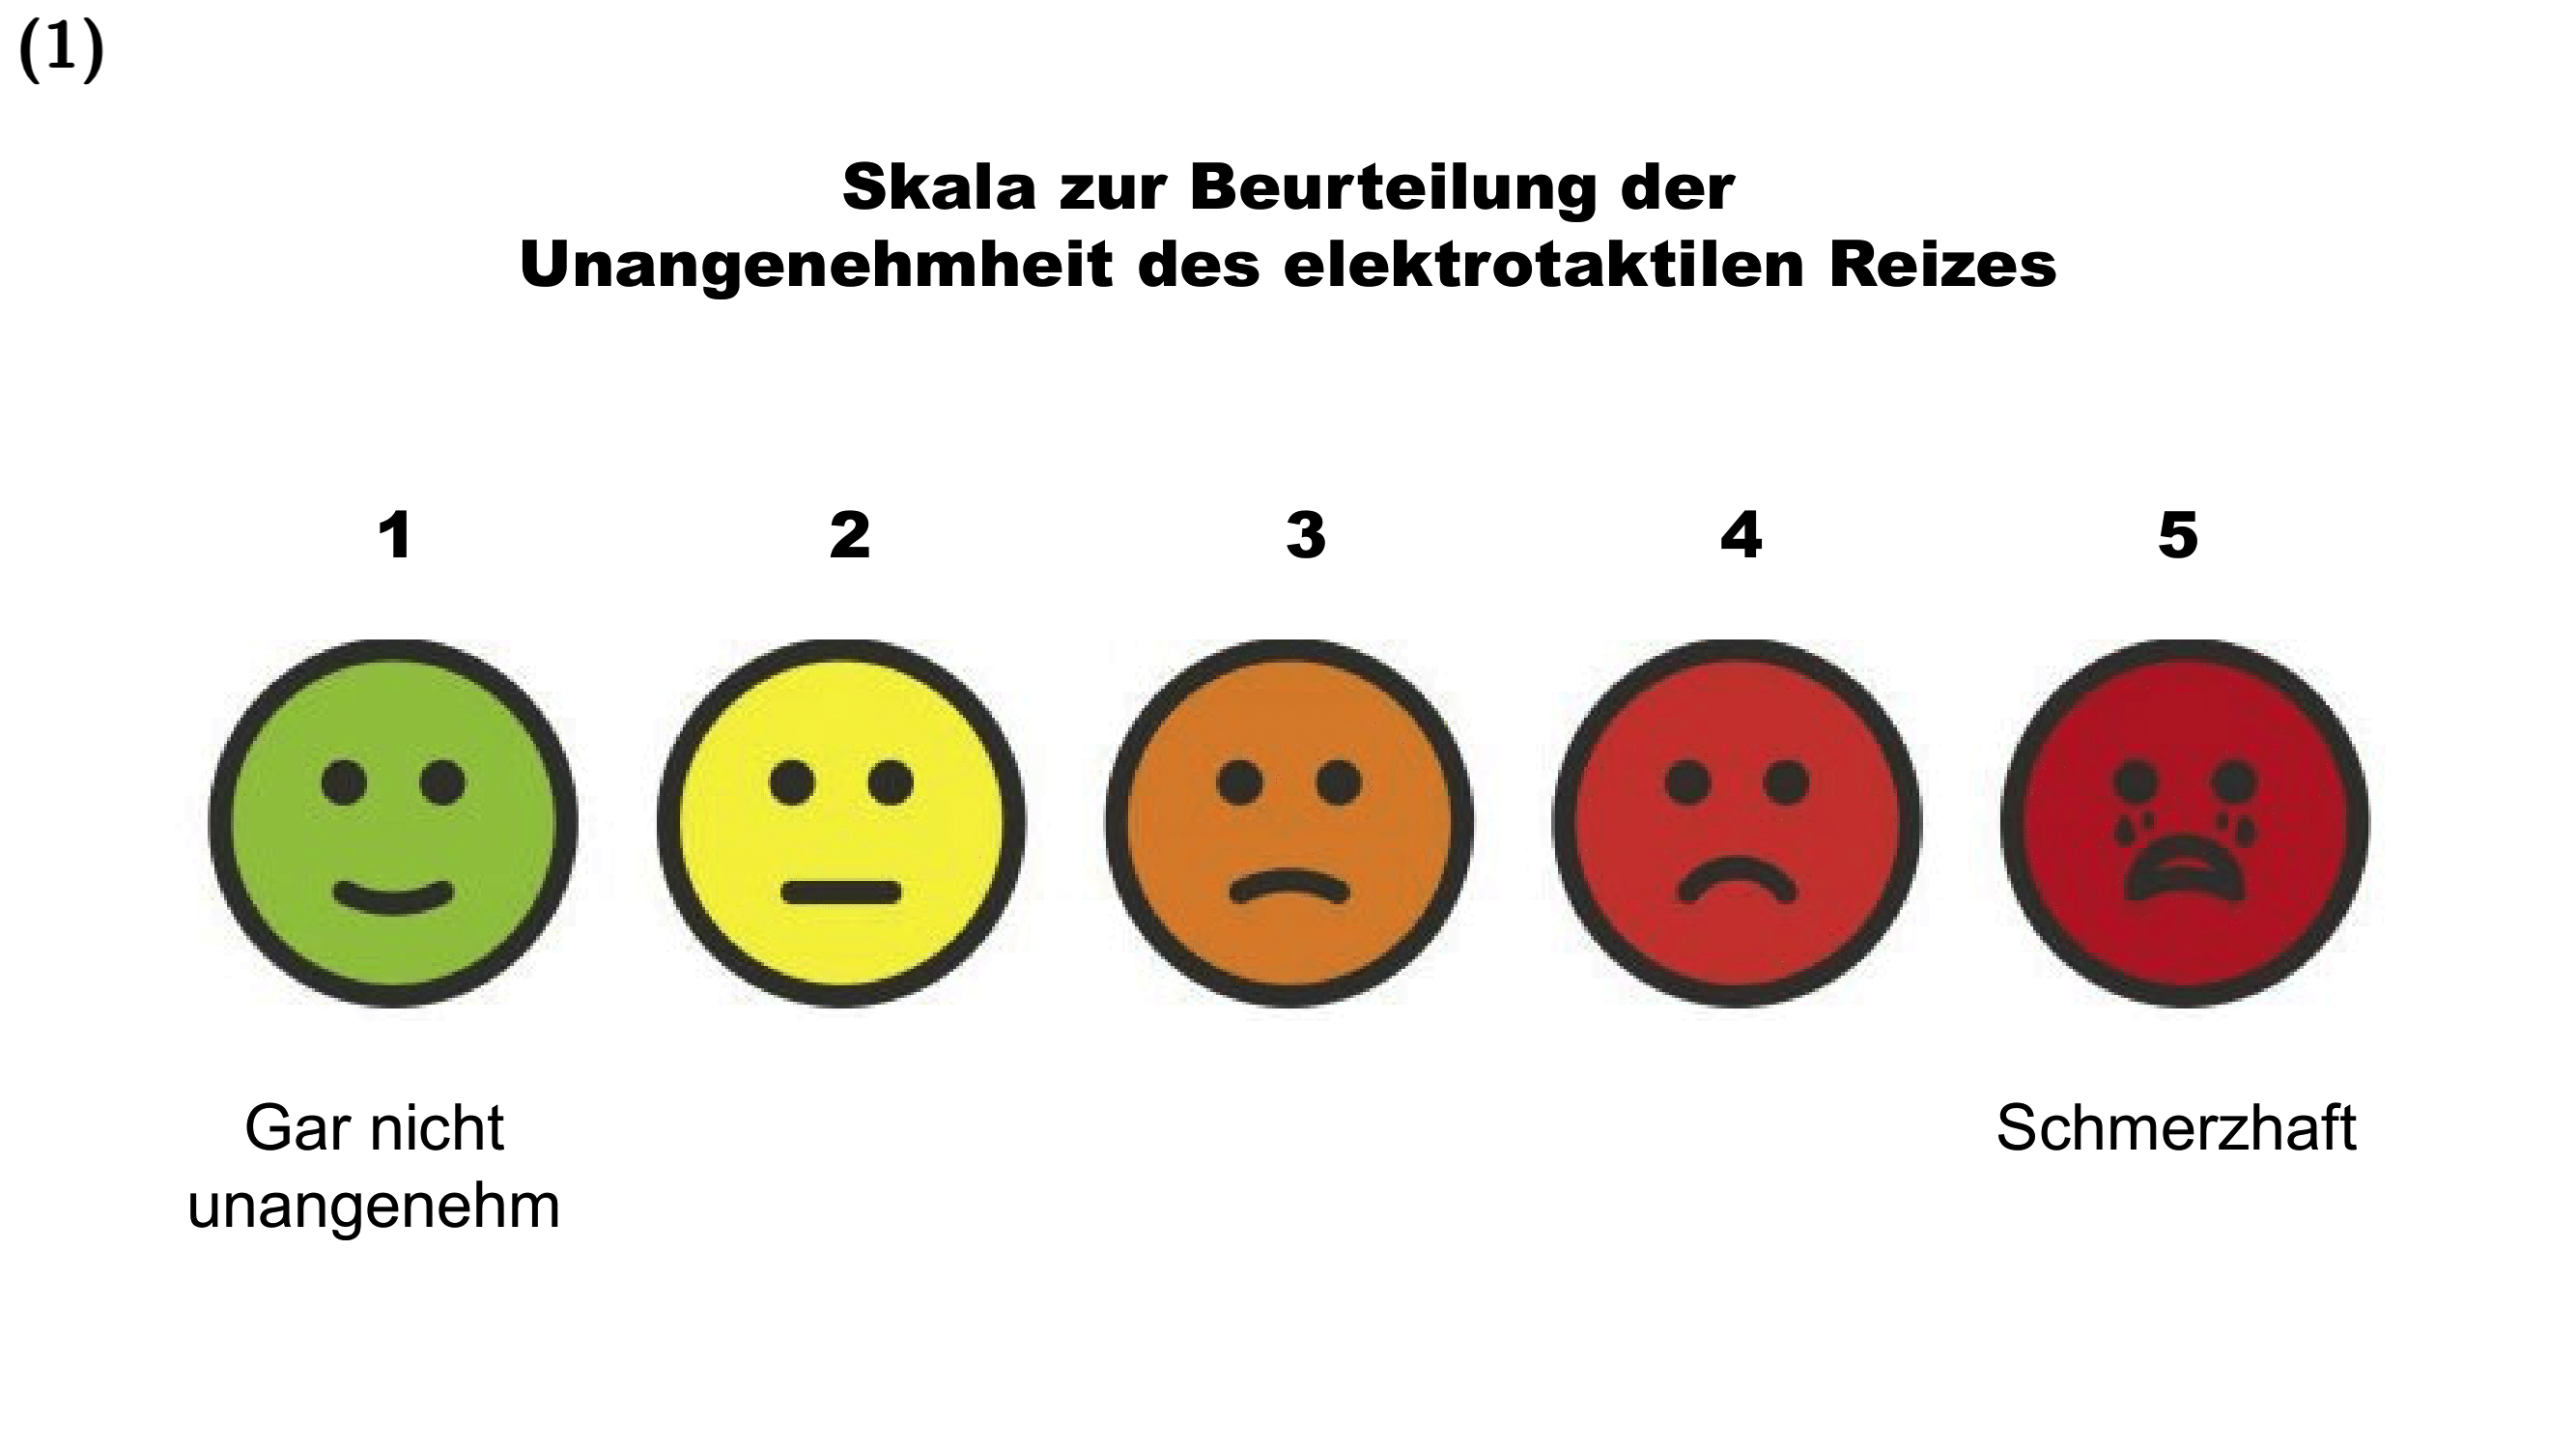
\includegraphics[width=\textwidth]{us_skala1.png}
	\end{minipage}

	\vspace*{1cm}
	\noindent\begin{minipage}[t]{14cm}
		\vspace*{0.5cm}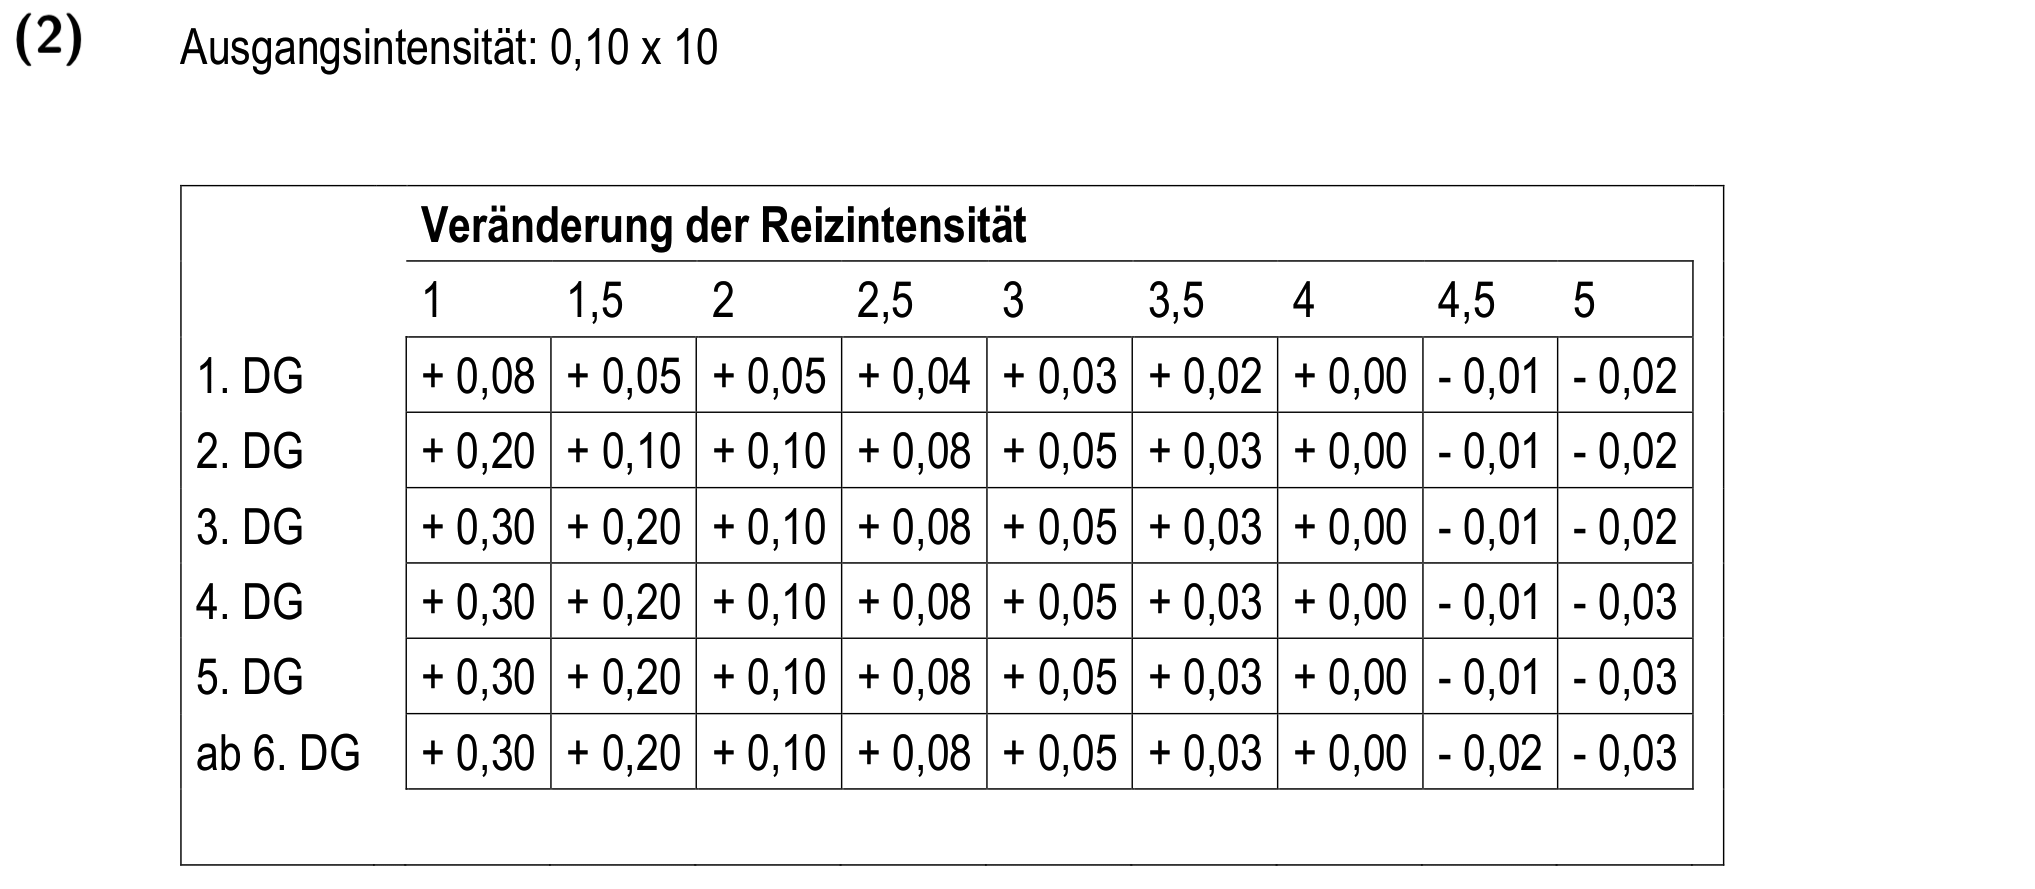
\includegraphics[width=\textwidth]{swu_tabelle1.png} 
	\end{minipage}
	\newpage
	

\section*{Anhang B} \label{appB}
	
	\noindent\textit{SAM-Skalen zur Einschätzung von Valenz und Erregung \parencite{BRADLEY1994}, deutsch adaptierte Fassung}
		
		\begin{minipage}[t]{0.95\textwidth}
			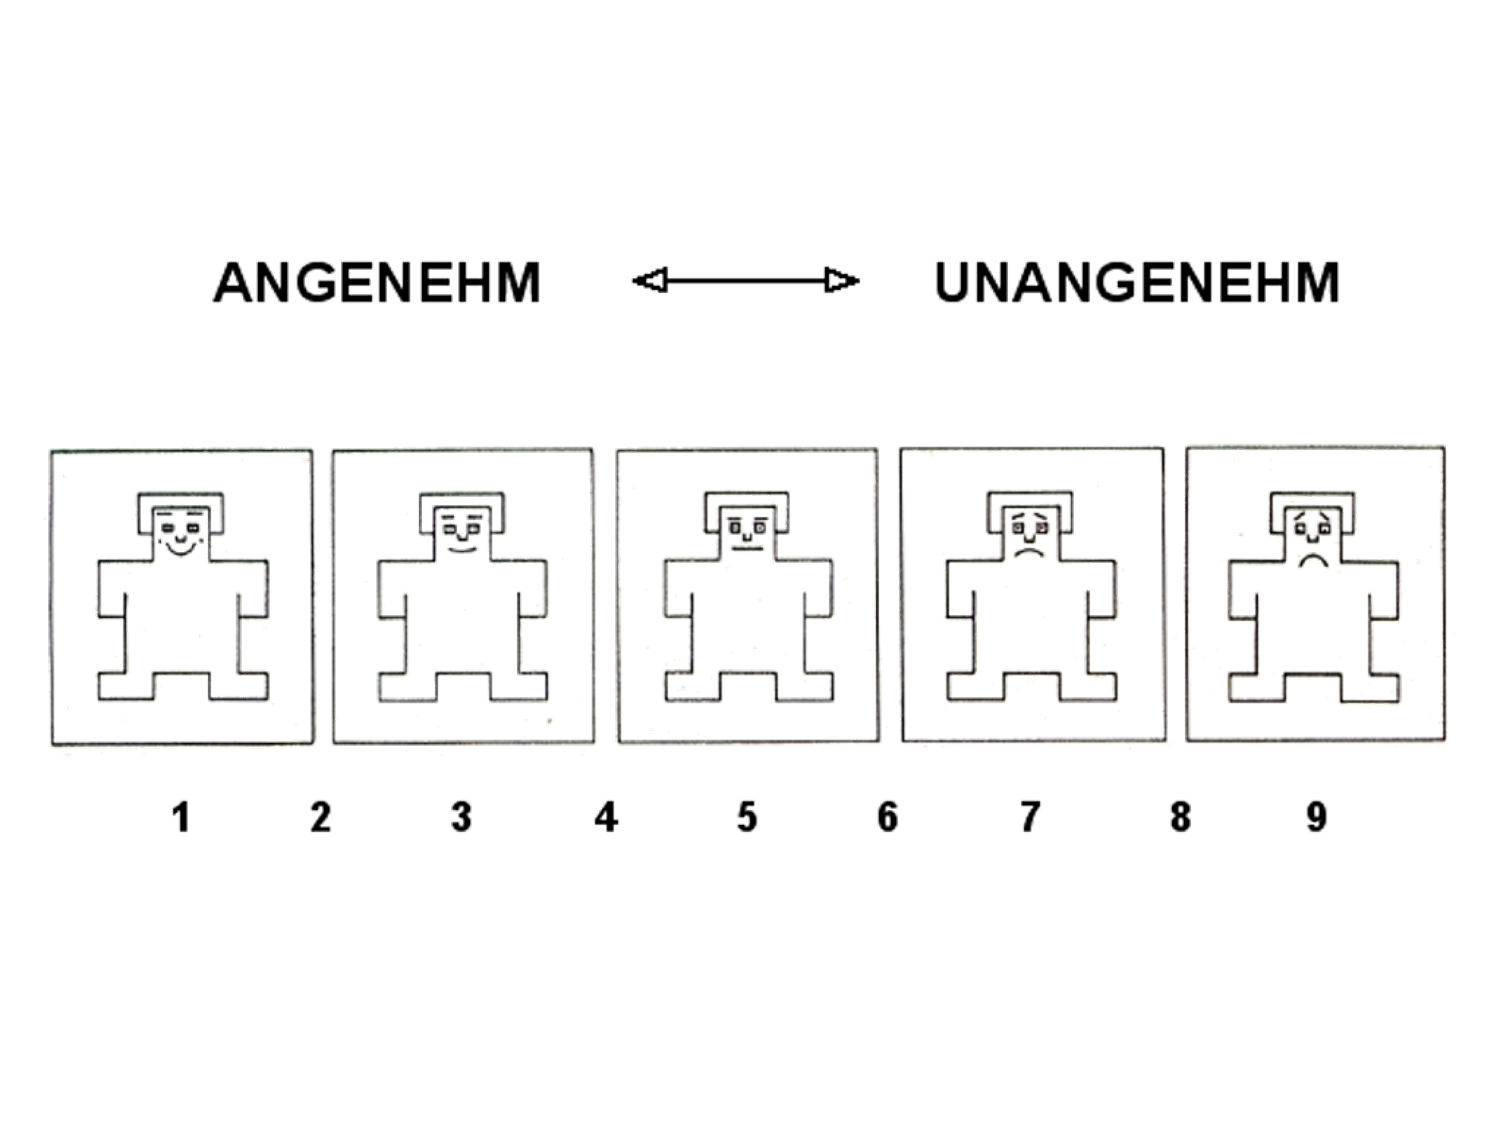
\includegraphics[width=0.9\textwidth]{SAM1} \vspace*{-1cm}
			
			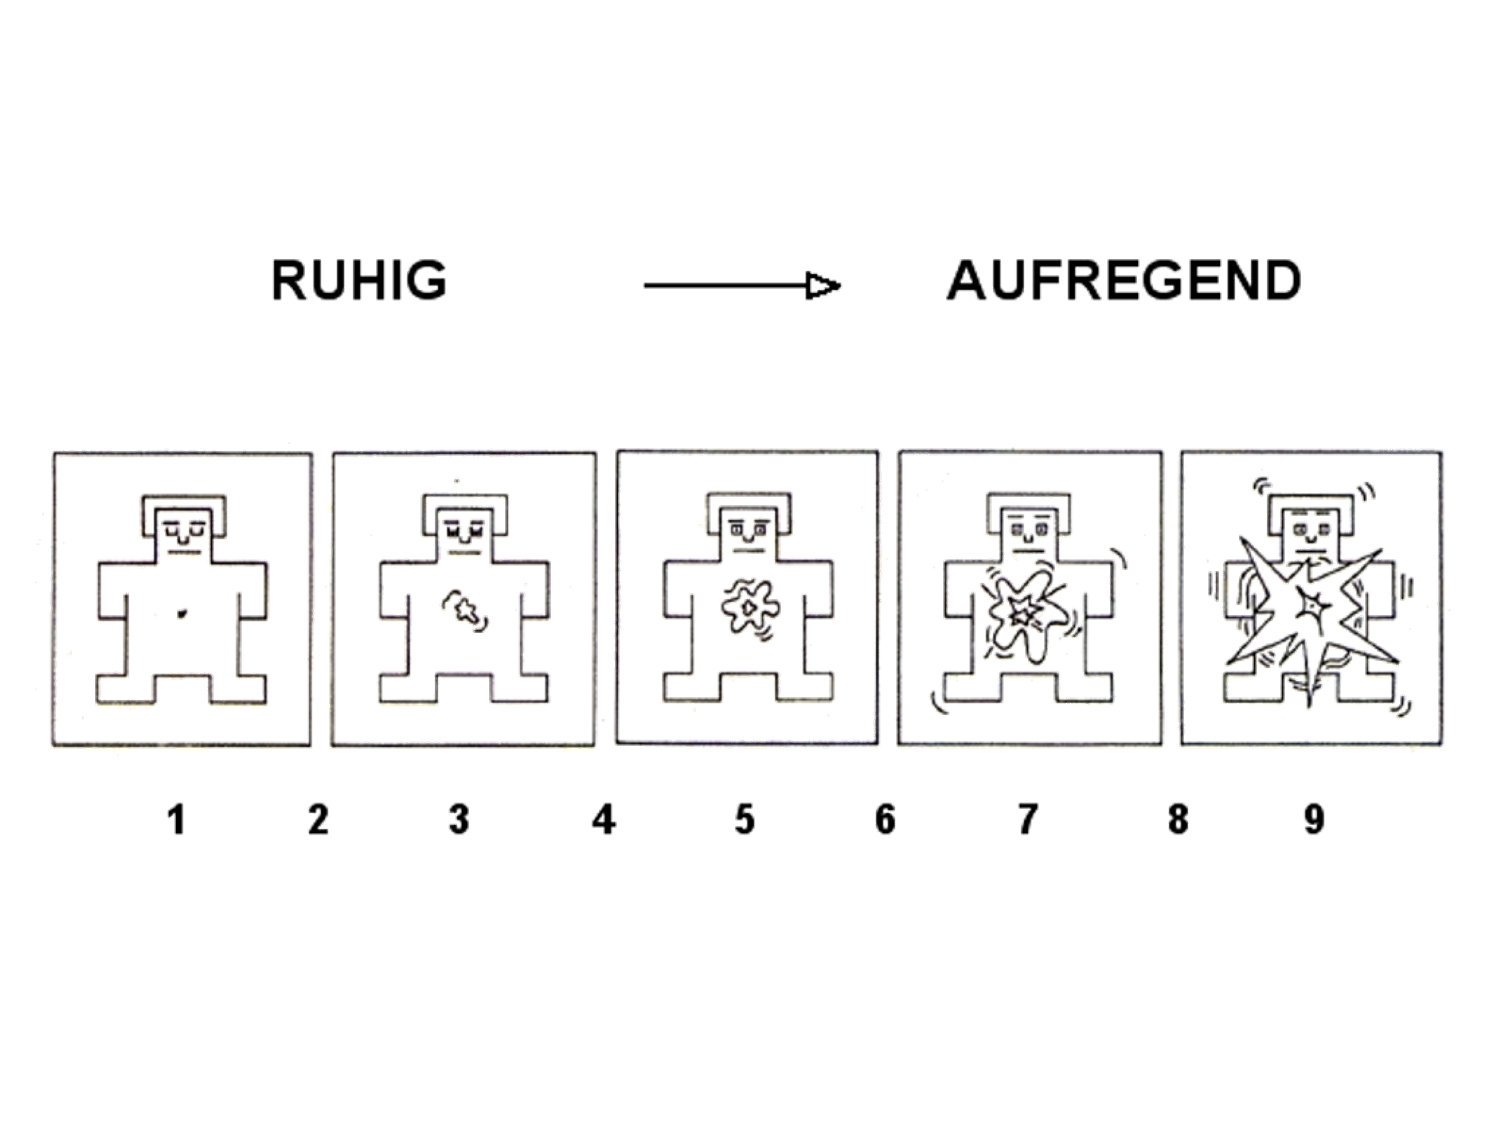
\includegraphics[width=0.9\textwidth]{SAM2}
		\end{minipage}
	\newpage


\section*{Anhang C} \label{appC}
	
	\noindent\textit{Streudiagramm zwischen Hautleitwert- und Schreckreaktionen. Die Gerade entspricht der Vorhersage eines einfachen linearen Modells mit \SI{95}{\percent}-Konfidenzgrenze}
		
		\vspace*{2cm}\hspace*{-0.5cm}
		\begin{minipage}[t]{0.95\textwidth}
			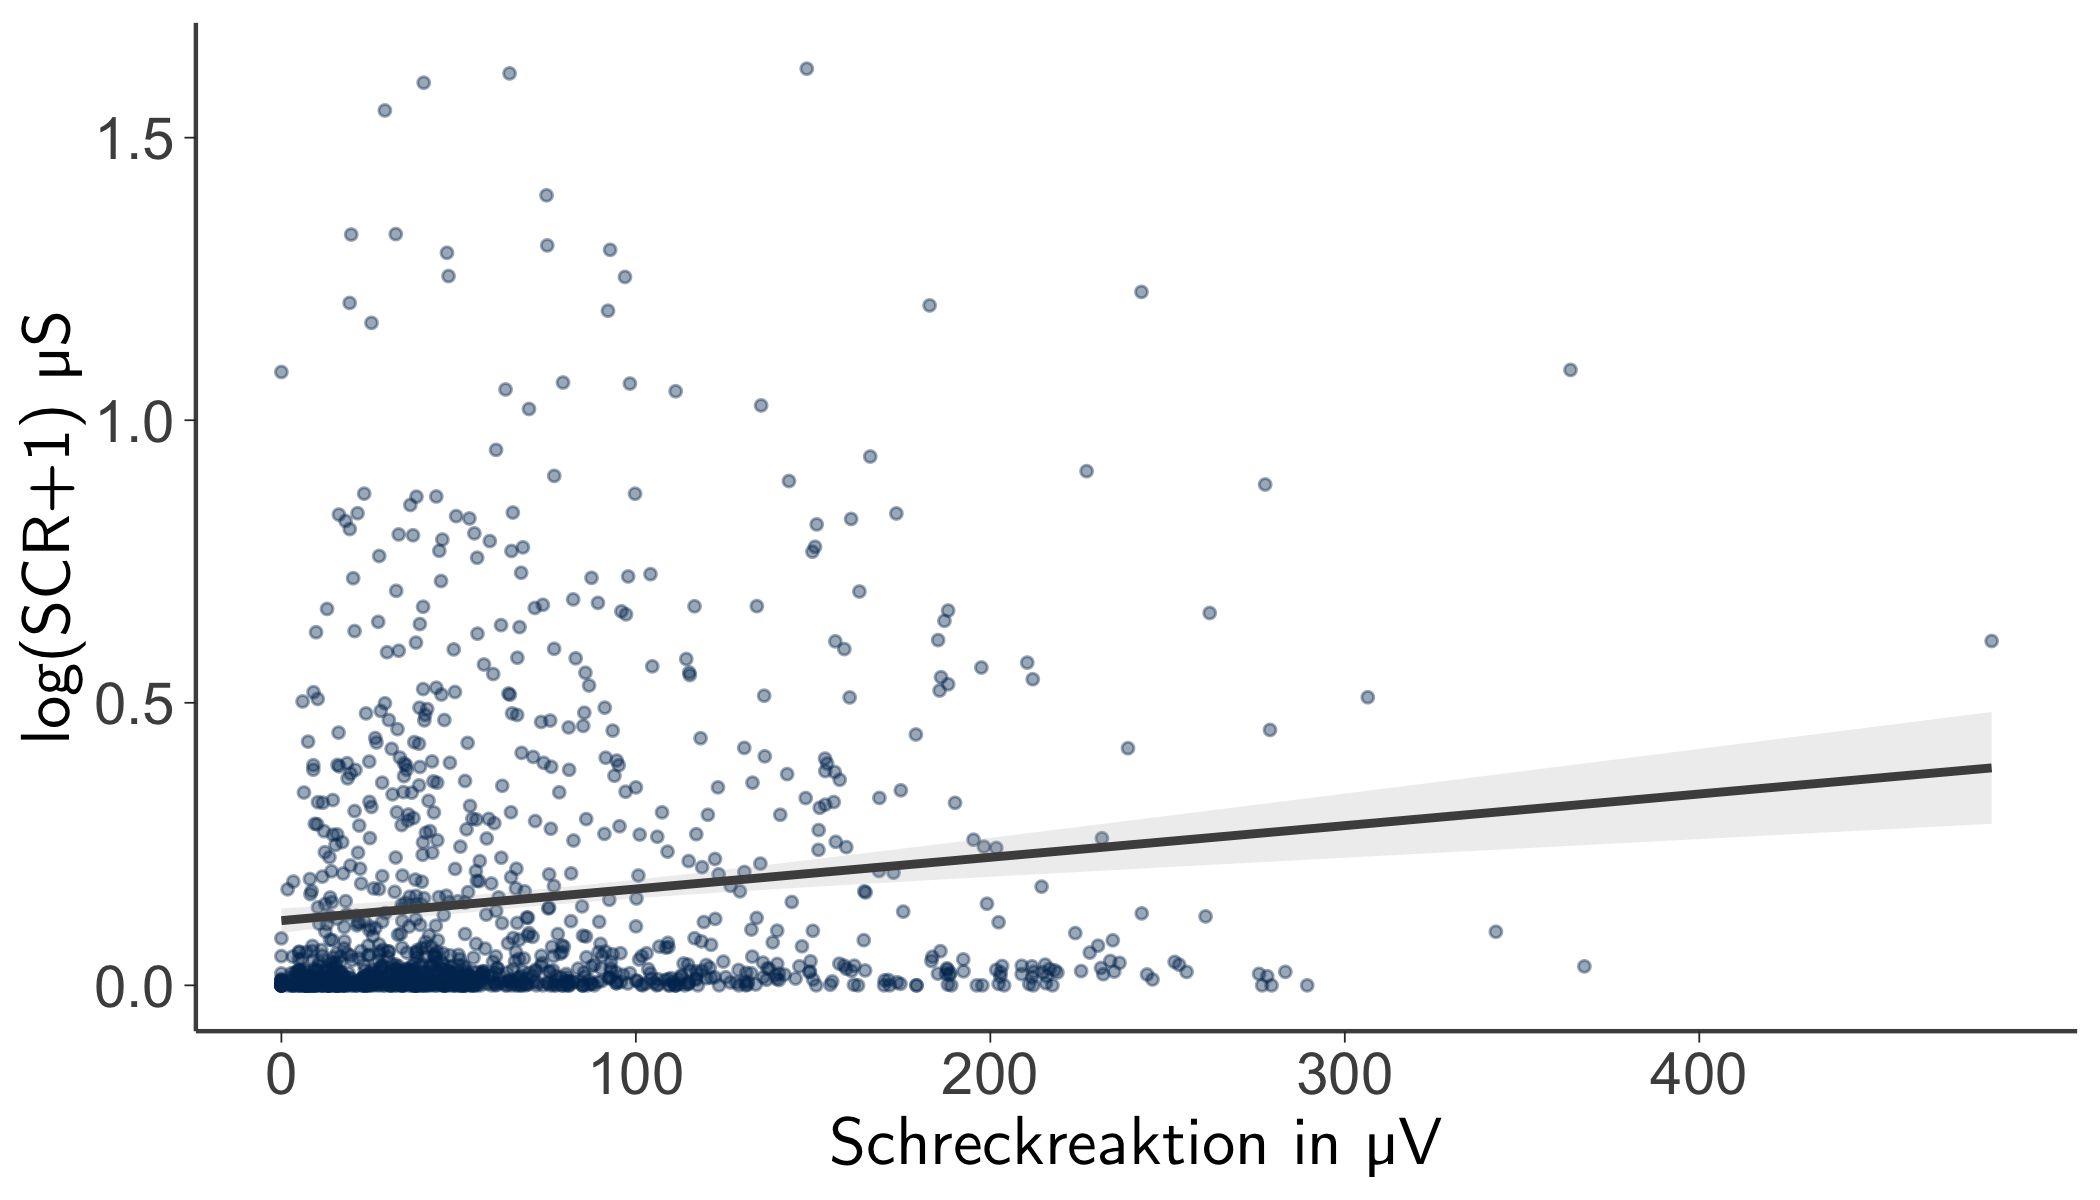
\includegraphics[width=0.9\textwidth]{multivariat1.png}
		\end{minipage}

	\newpage

\section*{Anhang D} \label{appD}

	\noindent \textit{Teststatistiken der Shapiro-Wilk-Tests für beide abhängigen Variablen}

	%\begin{table}[h]
	\vspace*{0.3cm}
		\begin{threeparttable}
			\begin{tabularx}{0.7\textwidth}{XCC}   \toprule
			 	Trial      	& SCR		 	& STR		\\ \hline \rowcolor[HTML]{EFEFEF}
			 	insgesamt  	& $0.64^{***}$		& $0.84^{***}$	\\
			 	 1 		& $0.81^{***}$  	& $0.81^{***}$	\\\rowcolor[HTML]{EFEFEF}
			 	 2 		& $0.68^{***}$  	& $0.91^{***}$	\\
			 	 3 		& $0.76^{***}$  	& $0.89^{***}$	\\\rowcolor[HTML]{EFEFEF}
			 	 4 		& $0.60^{***}$  	& $0.89^{***}$	\\
			 	 5 		& $0.61^{***}$  	& $0.87^{***}$	\\\rowcolor[HTML]{EFEFEF}
			 	 6 		& $0.67^{***}$  	& $0.77^{***}$	\\
			 	 7 		& $0.64^{***}$  	& $0.85^{***}$	\\\rowcolor[HTML]{EFEFEF}
			 	 8 		& $0.49^{***}$  	& $0.82^{***}$	\\
			 	 9  	& $0.78^{***}$  	& $0.82^{***}$	\\\rowcolor[HTML]{EFEFEF}
			 	 10 	& $0.66^{***}$  	& $0.79^{***}$  \\
			 	 11 	& $0.64^{***}$  	& $0.79^{***}$	\\\rowcolor[HTML]{EFEFEF}
			 	 12 	& $0.59^{***}$  	& $0.83^{***}$	\\
			 	 13 	& $0.59^{***}$  	& $0.86^{***}$	\\\rowcolor[HTML]{EFEFEF}
			 	 14 	& $0.62^{***}$  	& $0.80^{***}$	\\
			 	 15 	& $0.59^{***}$  	& $0.75^{***}$	\\\rowcolor[HTML]{EFEFEF}
			 	 16 	& $0.53^{***}$  	& $0.82^{***}$	\\\bottomrule
			\end{tabularx}
			\begin{tablenotes}[normal, flushleft, para]
				\footnotesize{\item \textit{Anmerkungen.} SCR: Hautleitwertreaktion, STR: Schreckreaktion; \\ ${}^{*}\, p<.05$, ${}^{**}\, p<.01$, ${}^{***}\, p<.001$.}
			\end{tablenotes}
		\end{threeparttable}
	%\end{table}		
	\newpage



\section*{Anhang E} \label{appE}

	\noindent\textit{Streudiagramme (und Korrelationen) zwischen den geschätzten zufälligen Effekten beider abhängiger Variablen}
	
	\vspace*{1cm}\hspace*{-0.5cm}
	\begin{minipage}{\textwidth}
			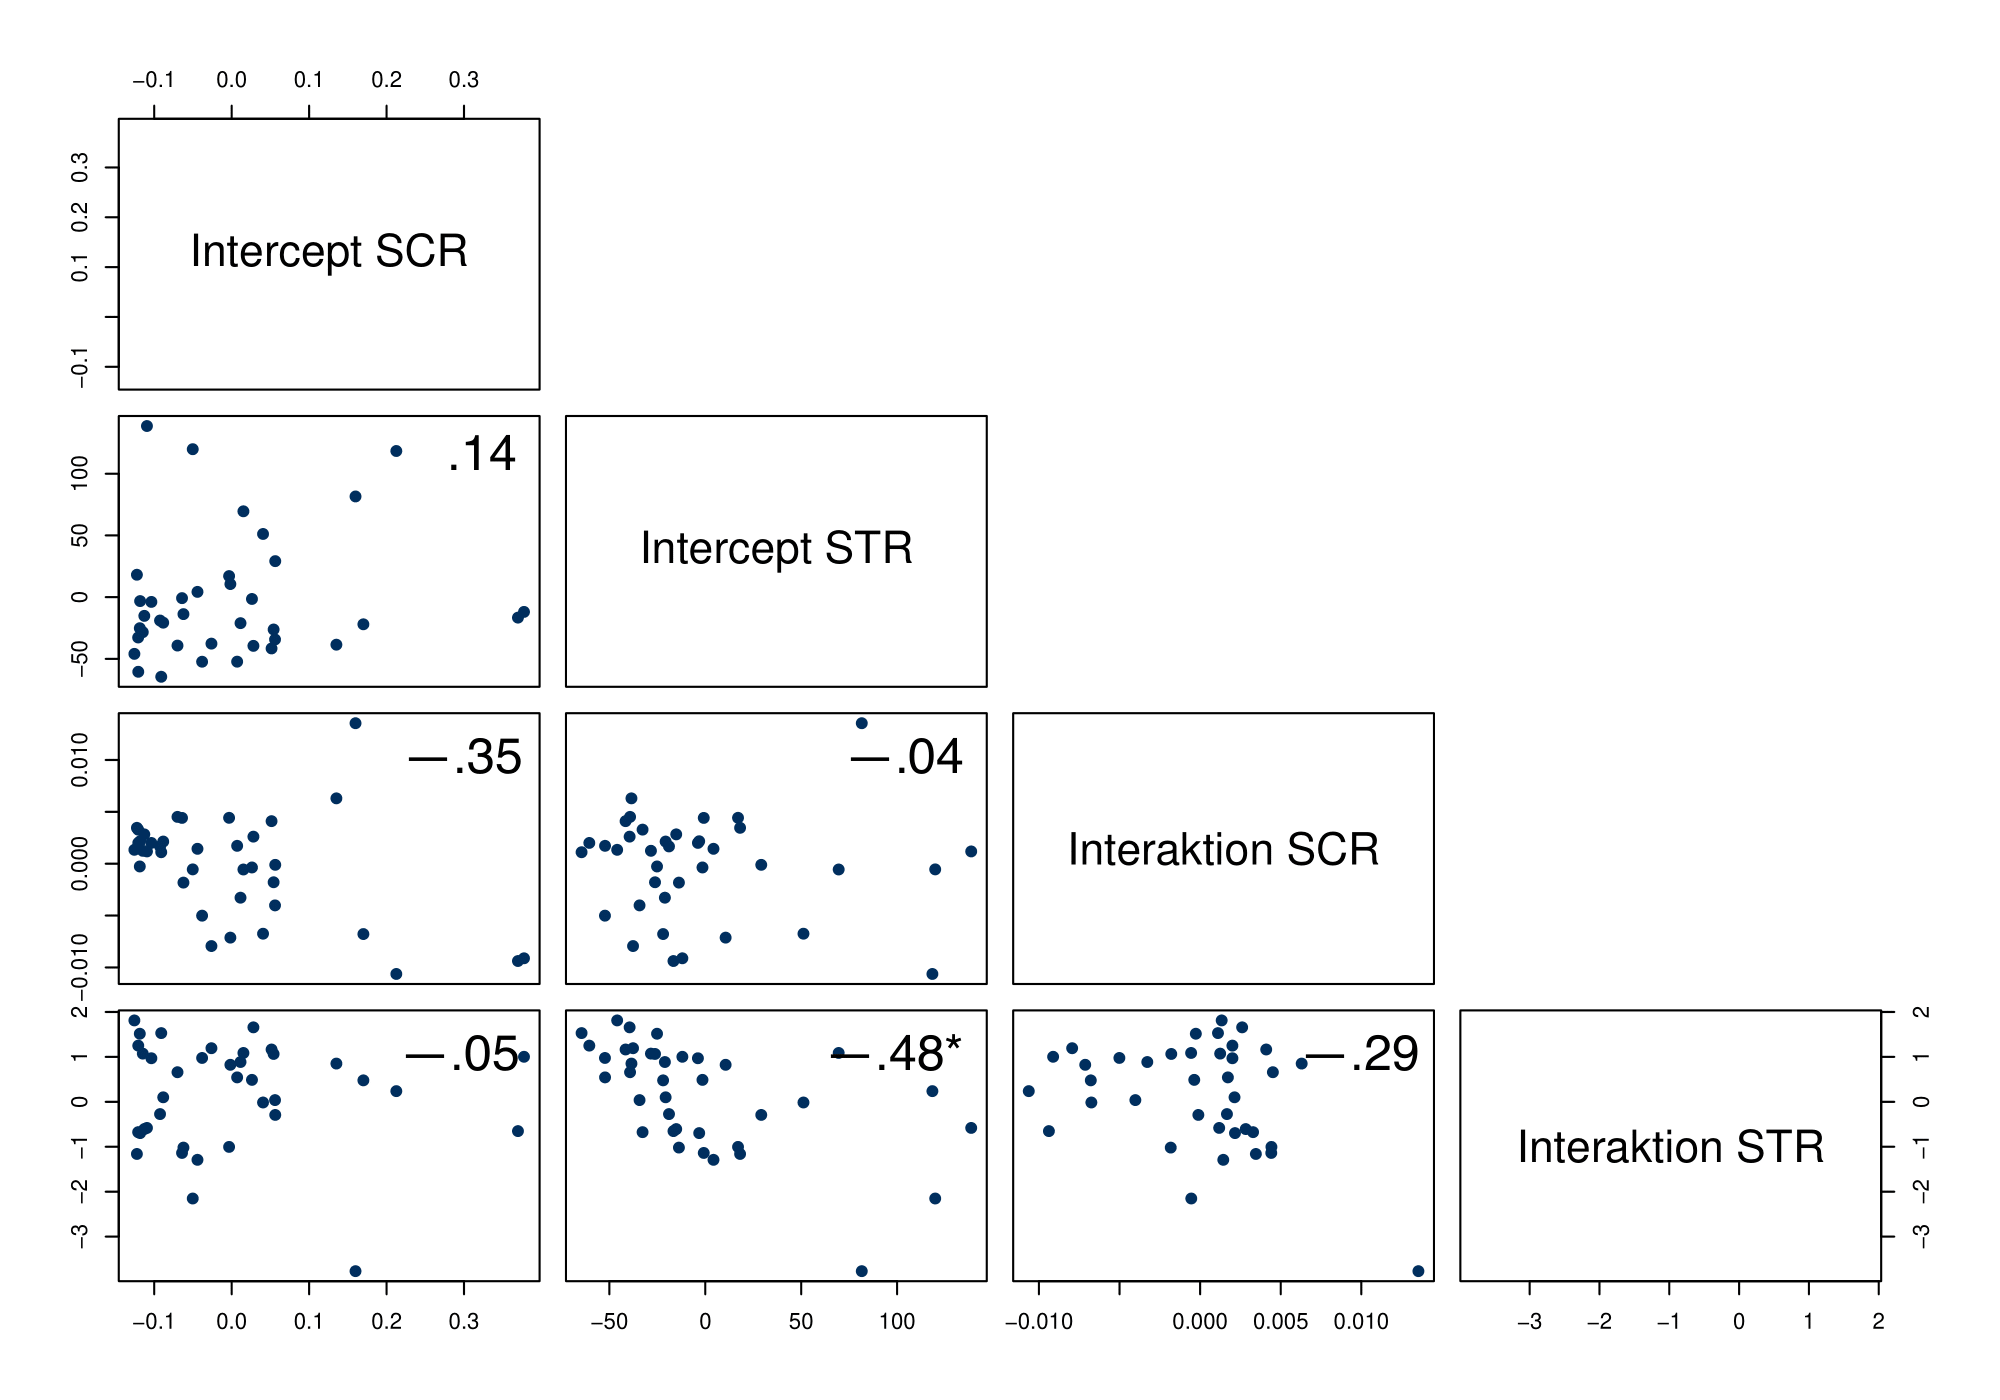
\includegraphics[width=\textwidth]{rescatter2.png}
	\end{minipage}


\section*{Anhang F} \label{appF}

\noindent\textit{Streudiagramme zwischen Residuen der höchsten Gruppierungsebene und angepassten Werten für beide AV (\textbf{a}, \textbf{b}) sowie  Q-Q-Diagramme (\textbf{c}, \textbf{d}) und Histogramme (\textbf{e}, \textbf{f}) dieser Residuen für beide AV}

\vspace*{0.5cm}\hspace*{-0.5cm}
\begin{minipage}[t]{\textwidth}
			\begin{tikzpicture}[remember picture] \centering		
			\node[inner sep=0pt] (a1) at (0,0)
			{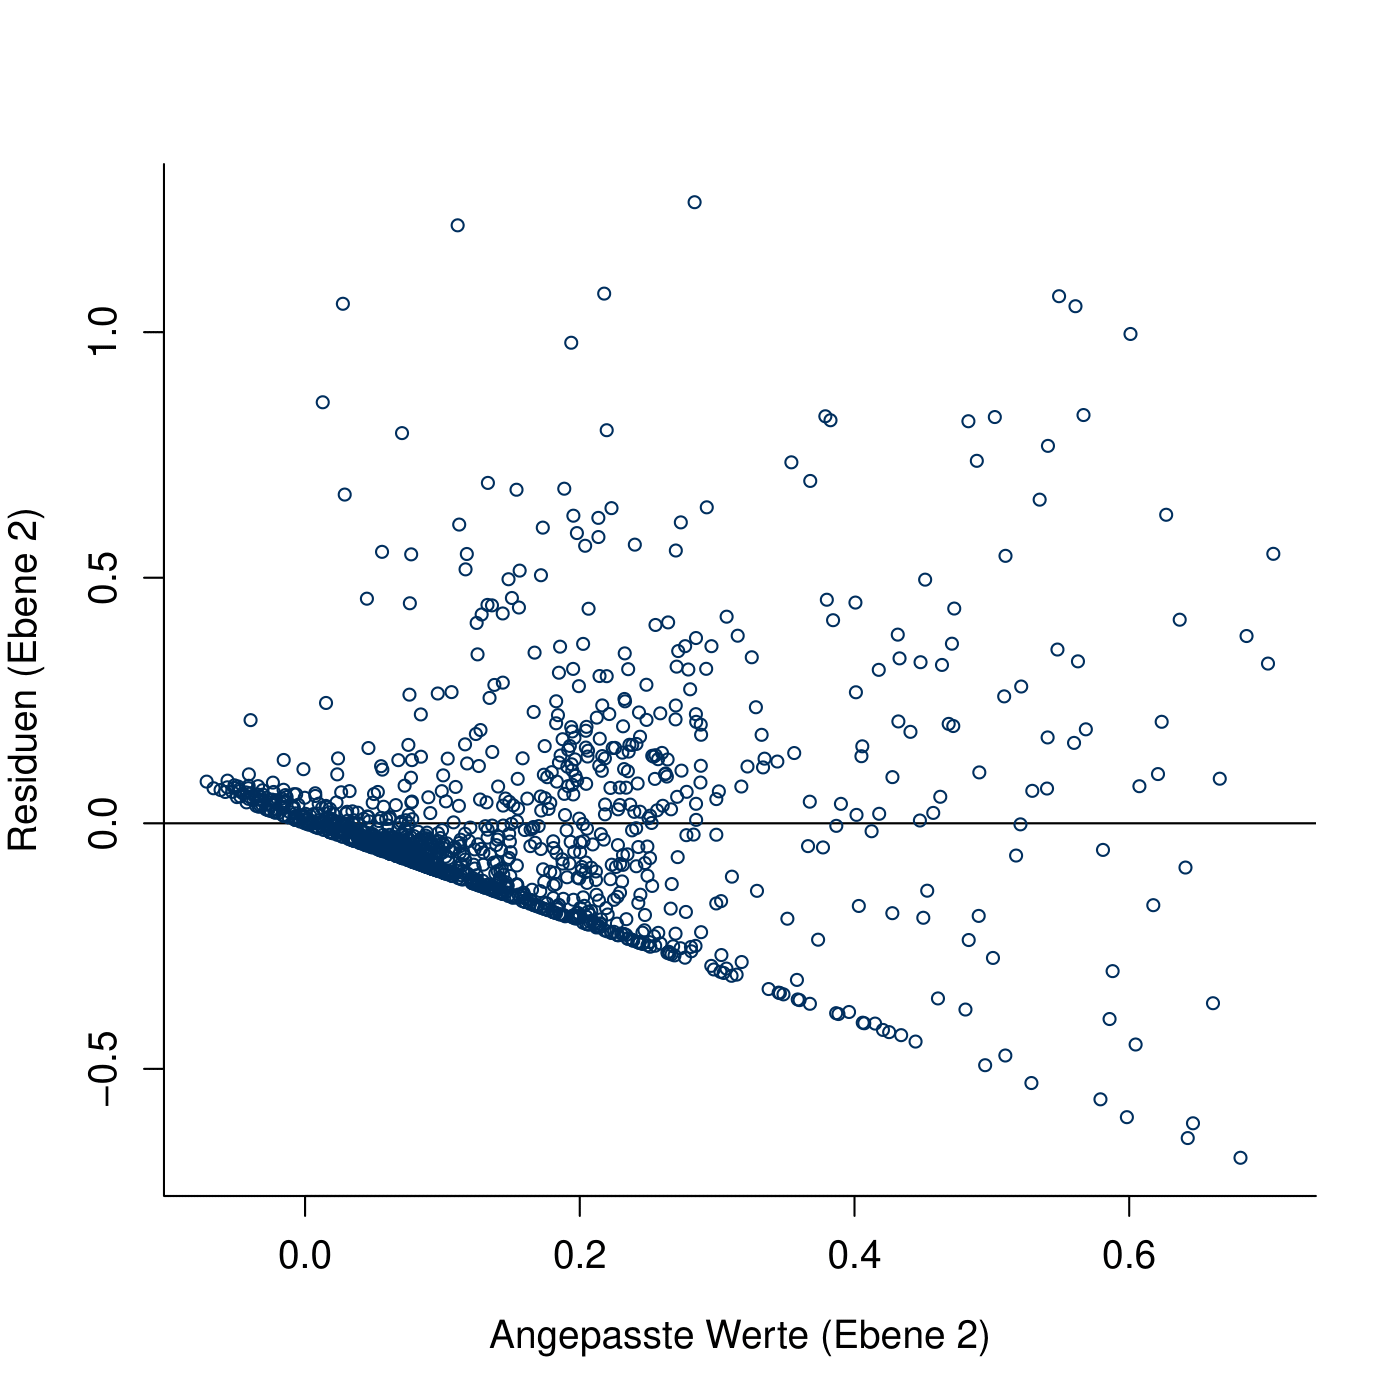
\includegraphics[scale=0.135]{as_scr_1.png}};
			\node[inner sep=0pt, right = 1cm of a1] (a2)
			{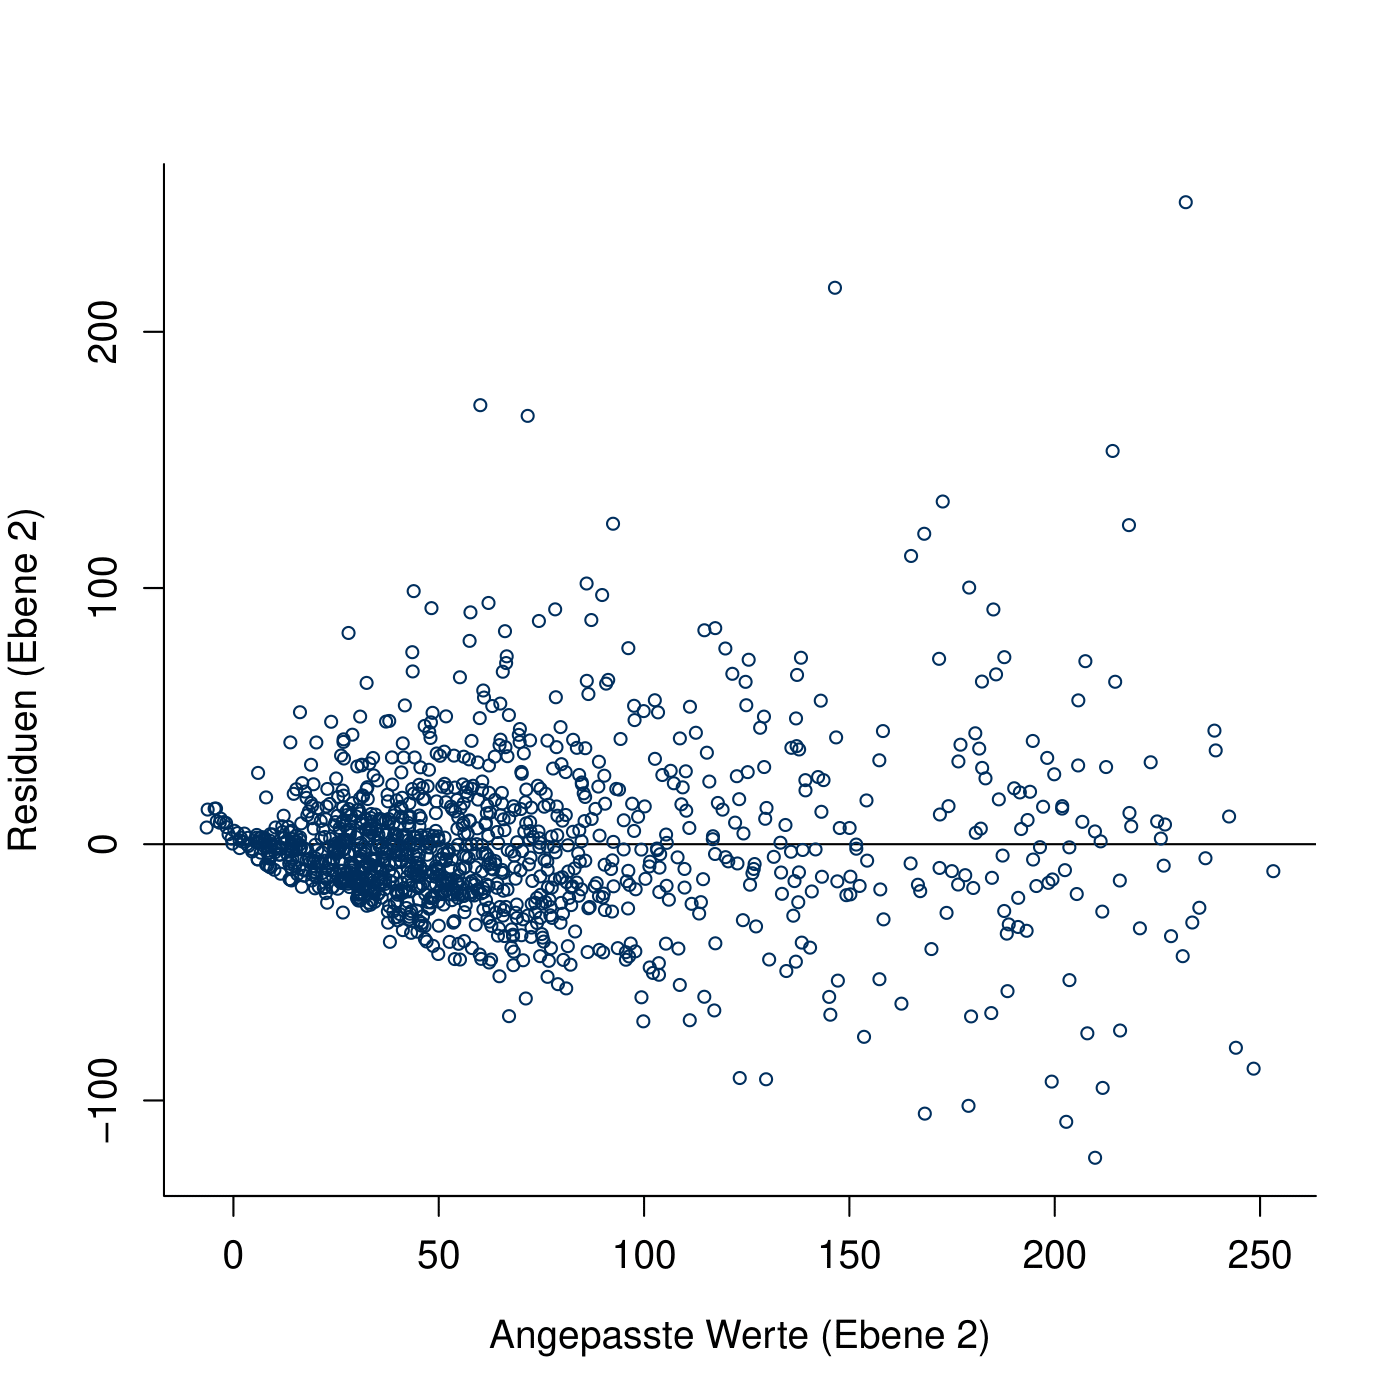
\includegraphics[scale=0.135]{as_str_1.png}};			
			\node[inner sep=0pt, below = 0.3cm of a1] (a3)
			{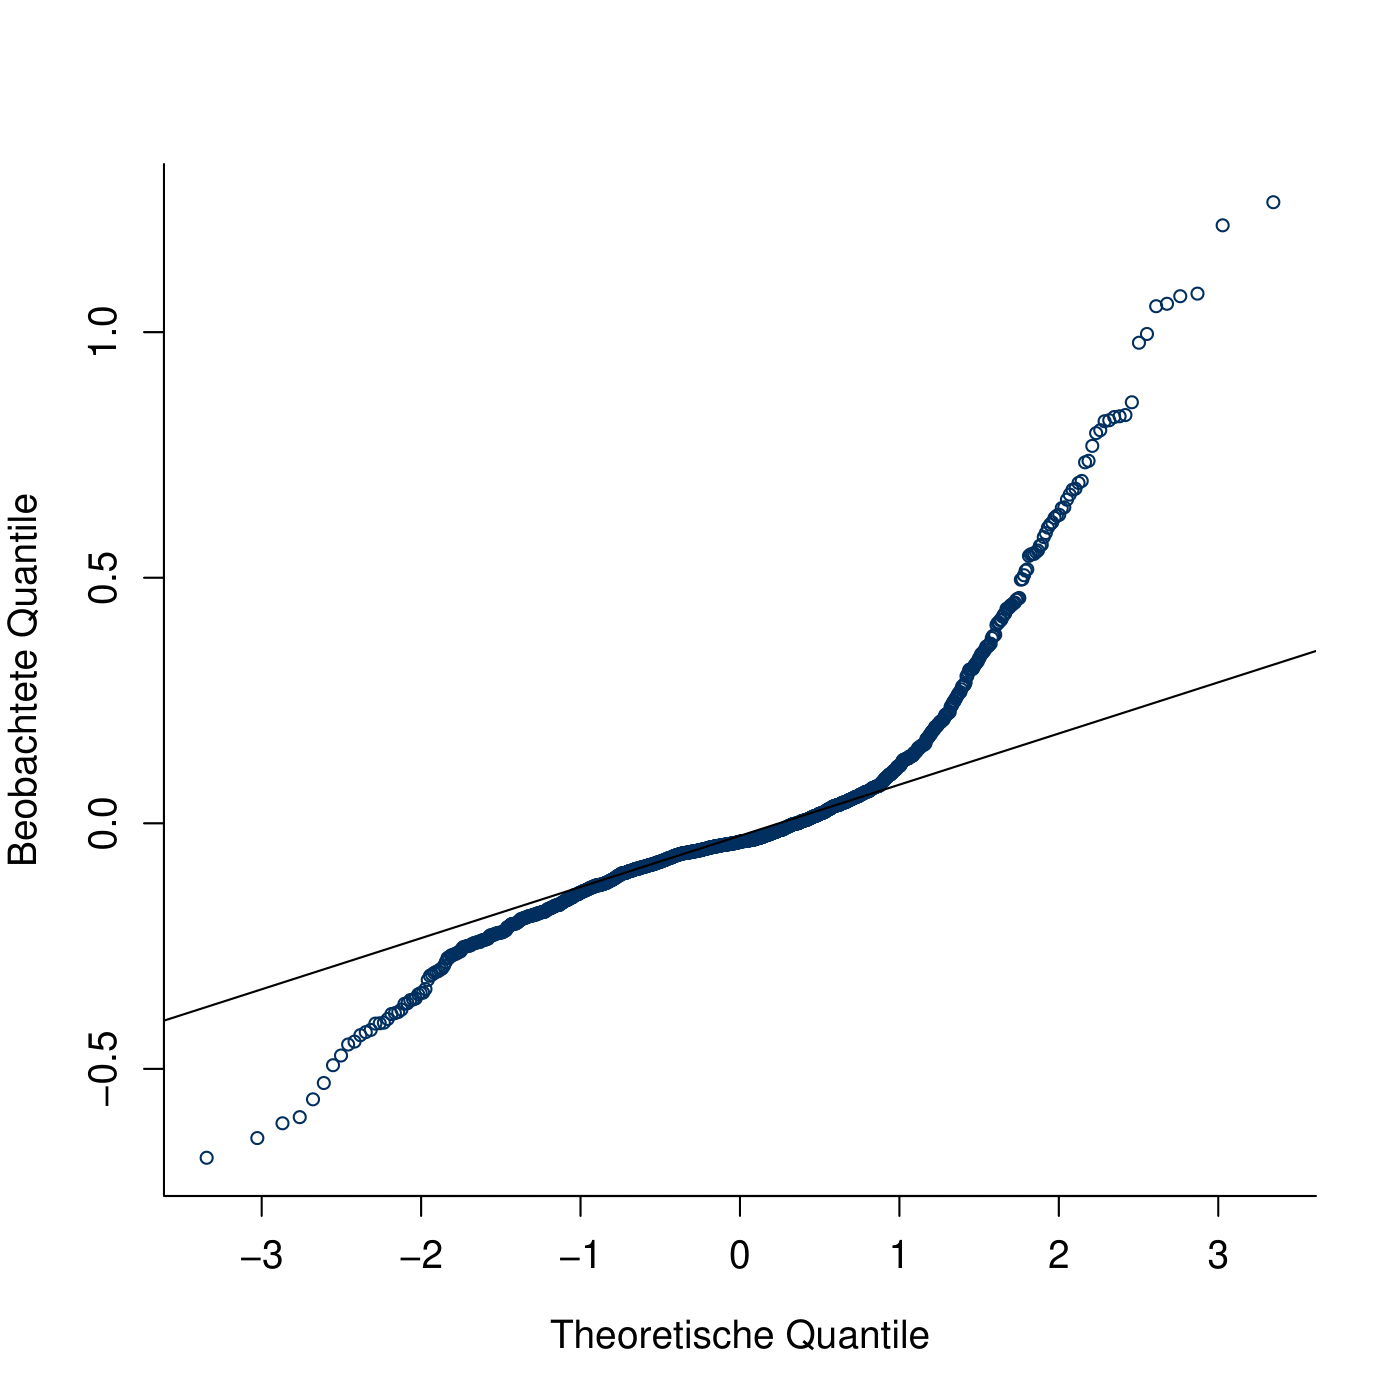
\includegraphics[scale=0.135]{qq_scr_1.png}};
			\node[inner sep=0pt, below = 0.3cm of a2] (a4)
			{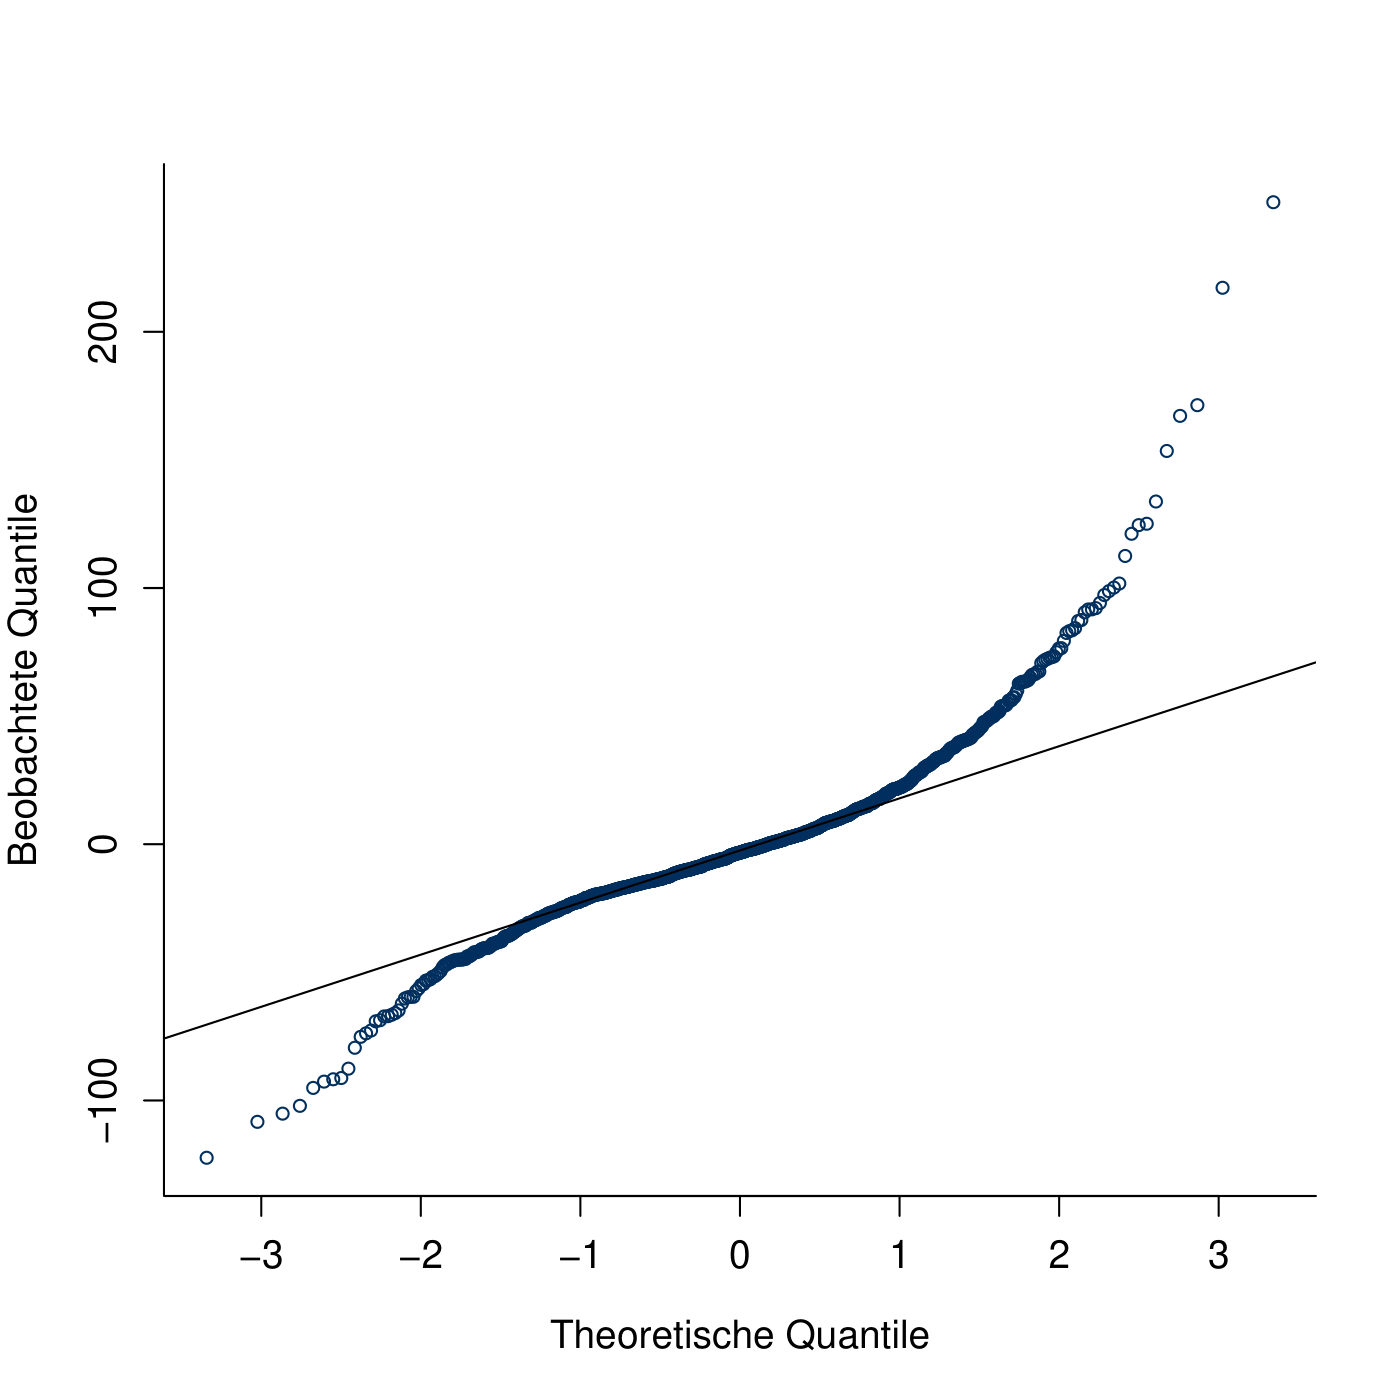
\includegraphics[scale=0.135]{qq_str_1.png}};
			\node[inner sep=0pt, below = 0.3cm of a3] (a5)
			{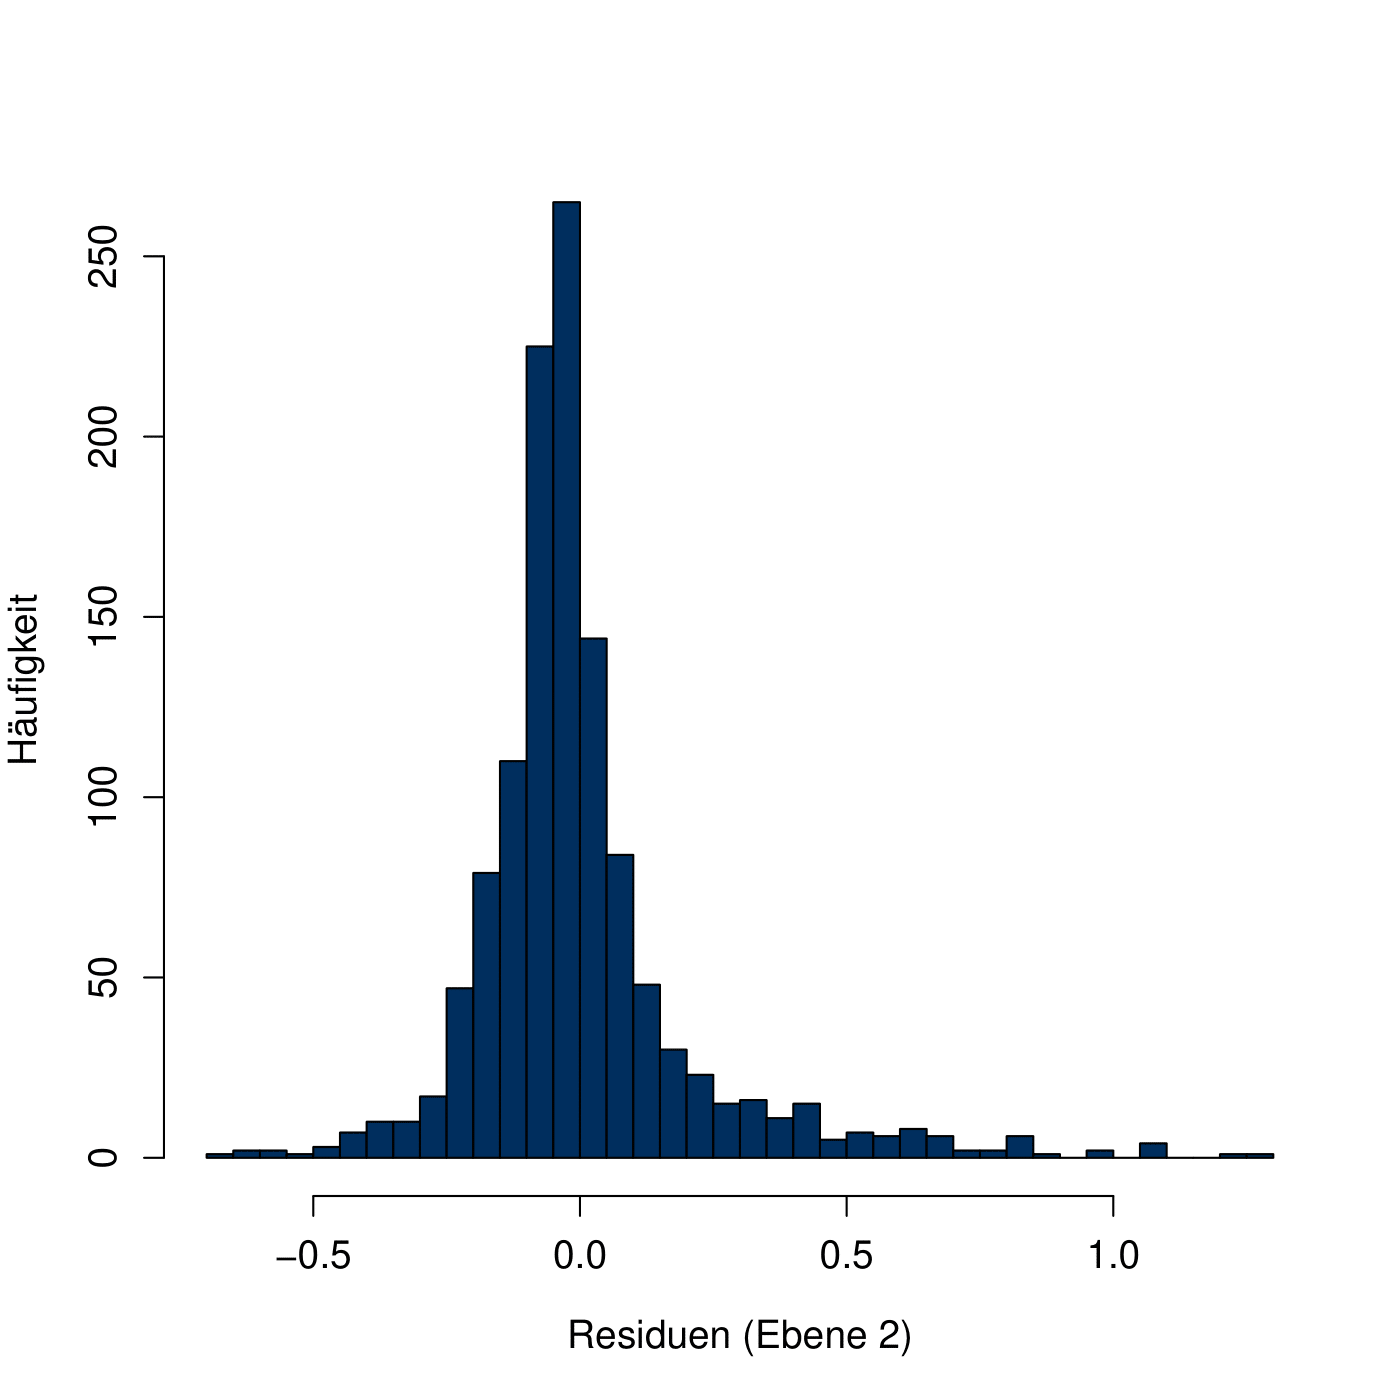
\includegraphics[scale=0.135]{his_scr_1.png}};
			\node[inner sep=0pt, below = 0.3cm of a4] (a6)
			{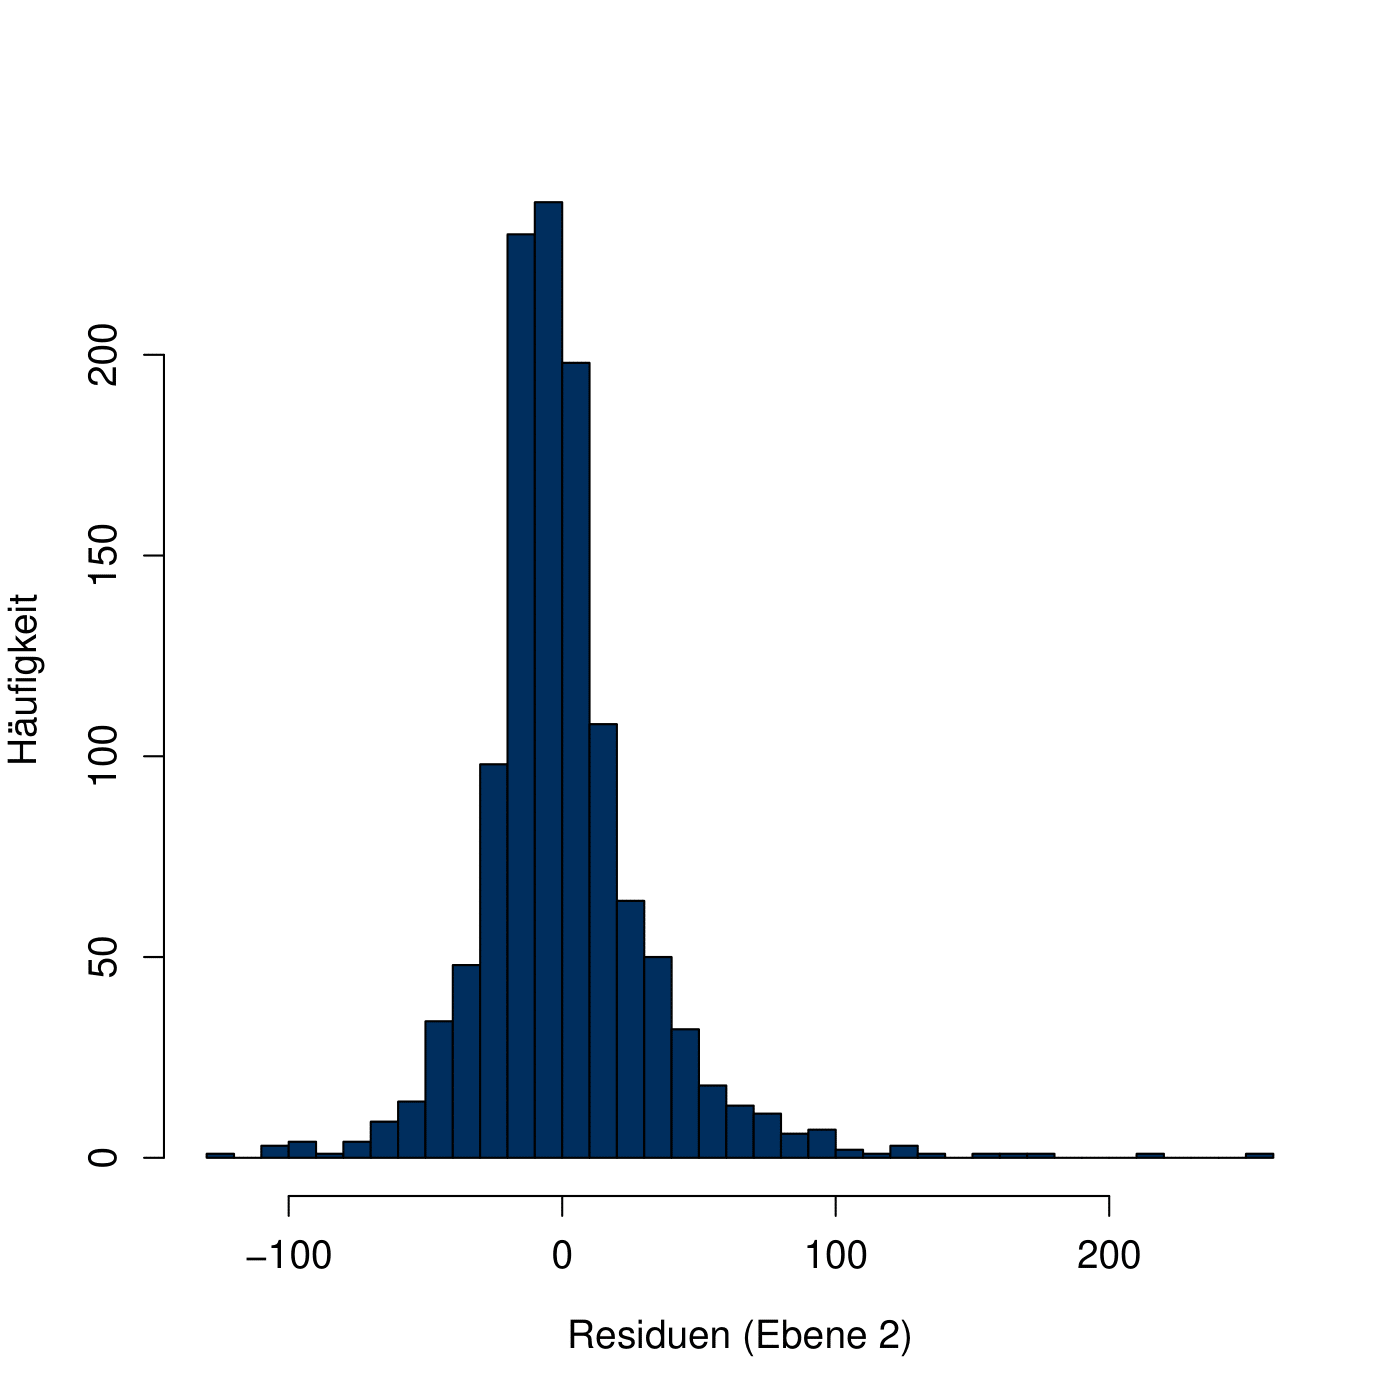
\includegraphics[scale=0.135]{his_str_1.png}};
			\node[above = 0.3cm of a1] (SCR) {\large{\textsf{\textbf{SCR}}}};
			\node[above = 0.3cm of a2] (STR) {\large{\textsf{\textbf{STR}}}};
			\node[above left = 0cm and -0.5cm of a1] (a) {\large{\textsf{\textbf{a}}}};
			\node[above left = 0cm and -0.5cm of a2] (b) {\large{\textsf{\textbf{b}}}};
			\node[above left = 0cm and -0.5cm of a3] (c) {\large{\textsf{\textbf{c}}}};
			\node[above left = 0cm and -0.5cm of a4] (d) {\large{\textsf{\textbf{d}}}};
			\node[above left = 0cm and -0.5cm of a5] (e) {\large{\textsf{\textbf{e}}}};
			\node[above left = 0cm and -0.5cm of a6] (f) {\large{\textsf{\textbf{f}}}};
		\end{tikzpicture}
\end{minipage}

		
%		\begin{enumerate}
%			\item ...
%			\item R-Code auf Stick
%			\item Matlab Codes auf Stick
%		\end{enumerate}
	
	%\noindent\textit{Hygieneverordnung Departement 09.05.2020 (auf Stick?)}